\section{Neuronske mreže}

\subsection{Neuron}

Neuronske mreže nastale su kao rezultat pokušaja reprodukcije rada ljudskog mozga.

Osnovna gradivna jedinica ljudskog mozga jest neuron. Ljudski mozak sastavljen je od oko $10^11$ neurona kojih ima više od 100 vrsta i koji su shodno svojoj funkciji raspoređeni prema točno definiranom 
rasporedu. Svaki je neuron u prosjeku povezan s $10^4$ drugih neurona. Četiri su osnovna dijela neurona: tijelo stanice (soma), skup dendrita (ogranaka), aksona (dugačke cijevčice koje prenose električke poruke) i niza završnih članaka 

\begin{figure}[htb]
\centering
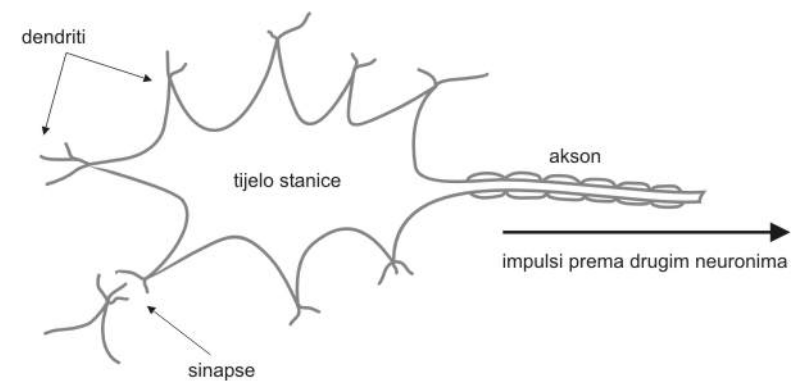
\includegraphics[width=8cm]{img/Neuron.png}
\caption{Građa neurona}
\label{img:human-neuron}
\end{figure}

Tijelo stanice sadrži informaciju predstavljenu električkim potencijalom između unutrašnjeg i vanjskog dijela stanice (oko –70 mV u neutralnom stanju). Na sinapsama, spojnom sredstvu dvaju neurona kojim su pokriveni dendriti, primaju se informacije od drugih neurona u vidu post-sinaptičkog potencijala koji utječe na potencijal stanice povećavajući (hiperpolarizacija) ili smanjivajući ga (depolarizacija). U tijelu stanice sumiraju se post-sinaptički potencijali tisuća susjednih neurona, u ovisnosti o vremenu dolaska ulaznih informacija. Ako ukupni napon pređe određeni prag, neuron "pali" i generira tzv. akcijski potencijal u trajanju od 1 ms. Kada se informacija akcijskim potencijalom prenese do završnih članaka, onda oni, ovisno o veličini potenijala, proizvode i otpuštaju kemikalije, tzv. neurotransmitere. To zatim ponovno inicira niz opisanih događaja u daljnjim neuronima. Propagacija impulsa očigledno je jednosmjerna. 

Funkcionalnost biološkog neurona imitira McCulloch-Pitts model umjetnog neurona, tzv. \textit{Threshold Logic Unit} (TLU). Model koristi slijedeću analogiju: signali su opisani numeričkim iznosom i na ulazu u neuron množe se težinskim faktorom koji opisuje jakost sinapse; signali pomnoženi težinskim faktorima zatim se sumiraju analogno sumiranju potencijala u tijelu stanice; ako je dobiveni iznos iznad definirana praga, neuron daje izlazni signal. 

U općenitom slučaju, umjetni neuron umjesto funkcije praga može imati i neku drugu funkciju, tzv. aktivacijsku funkciju (transfer funkcija, prijenosna funkcija). Općeniti model umjetnog neurona nalazi se na slici \ref{img:artificial-neuron}. U nastavku ćemo za pojam umjetni neuron ravnopravno koristiti i istovjetne pojmove: čvor ili jedinica. 

\begin{figure}[htb]
\centering
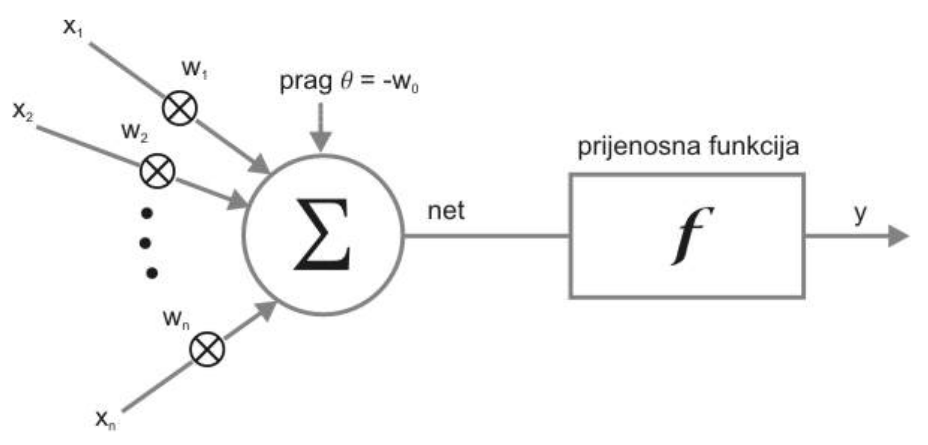
\includegraphics[width=8cm]{img/ArtificialNeuron.png}
\caption{Umjetni neuron}
\label{img:artificial-neuron}
\end{figure}

Ulazne signale (njih ukupno $n$) označavamo sa $x_1, x_2, x_3, ... , x_n$, a pripadajuće težine označavamo sa $\omega_1, \omega_2, \omega_3,..., \omega_n$.
Ulazni signali općenito su realni brojevi u intervalu $[-1,1]$, $[0,1]$ ili samo elementi iz $\{0,1\}$, kada govorimo o Booleovom ulazu. Težinska suma $net$ dana je formulom \ref{eq:weighted-sum}. Zbog kompaktnosti se često dogovorno uzima da je vrijednost praga $\theta = --\omega_0$ te se dodaje ulazni parametar $x_0$ s fiksiranom vrijednošću 1, te tada \ref{eq:weighted-sum} izgleda:

\begin{equation}
net = \omega_1 x_1 + \omega_2 x_2 + ... + \omega_n x_n - \theta
\label{eq:weighted-sum}
\end{equation}

\begin{equation}
net = \omega_0 x_0 + \omega_1 x_1 + \omega_2 x_2 + ... + \omega_n x_n = \sum_{i=0}^{n} \omega_i x_i
\label{eq:weighted-sum_2}
\end{equation}

Izlaz $y$ je rezultat aktivacijske funkcije te ga zapisujemo:

\begin{equation}
y = f(\sum_{i=0}^{n} \omega_i x_i) = f(net)
\label{eq:activation-function}
\end{equation}


\subsection{Svojstva umjetne neuronske mreže}

Umjetna neuronska mreža (\textit{engl.} Artificial Neural Network, ANN) u širem je smislu riječi umjetna replika ljudskog mozga kojom se nastoji simulirati postupak učenja. Nešto stroža definicija bila bi skup međusobno povezanih jednostavnih procesnih elemenata, \textit{jedinica} ili \textit{čvorova}, čija se funkcionalnost temelji na biološkom neuronu. Pri tome je obradbena moć mreže pohranjena u snazi veza između pojedinih neurona tj. težinama do kojih se dolazi postupkom prilagodbe odnosno učenjem iz skupa podataka za učenje. Neuronska mreža obrađuje podatke distribuiranim paralelnim radom svojih čvorova.

To je paradigma kojom su implementirani pojednostavljeni modeli što sačinjavaju biološku neuronsku mrežu. Ova je analogija vrlo poopćena jer, naravno, postoje još mnogi fenomeni živčanog sustava koji nisu modelirani ovim pristupom. Također, postoje i karakteristike umjetnih neuronskih mreža koje se ne poklapaju sa onima živčanog sustava.

Prednosti neuronskih mreža nad standardnim (simboličkim) načinom obrade podataka:

\begin{itemize}
\item Vrlo su dobre u procjeni nelineranih odnosa uzoraka
\item Mogu raditi s nejasnim ili manjkavim podacima tipičnim za podatke iz različitih senzora, poput kamera i mikrofona, i u njima raspoznavati uzorke
\item Robusne su na pogreške u podacima, za razliku od konvencionalnih metoda koje pretpostavljaju normalnu raspodjelu obilježja u ulaznim podacima
\item Stvaraju vlastite odnose između podataka koji nisu zadani na ekplicitan simbolički način
\item Mogu raditi s velikim brojem varijabli ili parametara
\item Prilagodljive su okolini
\item Moguća je jednostavna VLSI implementacija (\textit{engl.} Very-large-scale integration)
\item Sposobne su formirati znanje učeći iz iskustva (tj. primjera)
\end{itemize}

Neuronske mreže odlično rješavaju sve probleme kod kojih postoji odnos između prediktorskih (ulaznih) i zavisnih (izlaznih) varijabli, bez obriza na visoku složenost te veze (nelinearnost) -- \textit{klasifikacija} i \textit{regresija} (\textit{predviđanje}). Neuronske mreže uključuju se u sve više pordučja, a primjeri domena na kojima se već široko primjenjuju su:

\begin{itemize}
\item raspoznavanje uzoraka
\item obrada slike
\item obrada teksta
\item obrada govora (zvuka)
\item problemi optimizacije
\item nelinearno upravljanje
\item obrada nepreciznih i nekompletnih podataka
\item simulacije i mnogi drugi
\end{itemize}

Način na koji su neuroni međusobno organizirani i povezani u mreži određuju njezinu
arhitekturu. Razlikujemo četiri osnovne arhitekture:

\begin{itemize}
\item aciklička unaprijedna (\textit{engl. feedforward net}) mreža
\item mreža s povratnom vezom (\textit{engl. recurrent net})
\item lateralno povezana mreža
\item hibridna mreža
\end{itemize}

U ovom radu proučavat će se konvolucijske neuronske mreže koje spadaju u kategoriju unaprijednih acikličkih mreža. U konvolucijskim mrežama kao aktivacijske funkcije koriste se ReLu i sigmoidalna funkcija koje su opisane u nastavku.


\subsection{Aktivacijske funkcije}

\subsubsection{Adaline}

Adaline (\textit{engl. Adaptive Linear Element}) aktivacijska funkcija je prva aktivacijska funkcija ikada te dijeli ime sa neuronom koji ju koristi. Zbog svojeg ranog razvoja, naravno da je i najjednostavnija:

\begin{equation}
f(net) = net
\label{eq:Adaline aktivacijska funkcija}
\end{equation}

Izlaz iz takve jedinice upravo je težinska suma njegovih ulaza. Dakle, izlaz odgovara općenitom modelu umjetnog neurona prikazanom na slici \ref{img:artificial-neuron}, a dan je izrazom \ref{eq:activation-function}.

\subsubsection{Funkcija skoka}

Funkcija skoka ili praga (\textit{engl. Threshold Logic Unit, TLU}) na izlazu daje Booleov izlaz ($\{False, True\}, \{0, 1\}$). Graf TLU dan je slikom \ref{img:tlu}.

\begin{equation}
f(net)=\left\{
\begin{array}{c l}	
     0 & $\textit{za net} $ < $ $ 0,\\
     1 & $\textit{inače}$
\end{array}\right.
\label{eq:Funkcija skoka}
\end{equation}

\begin{figure}[H]
\centering
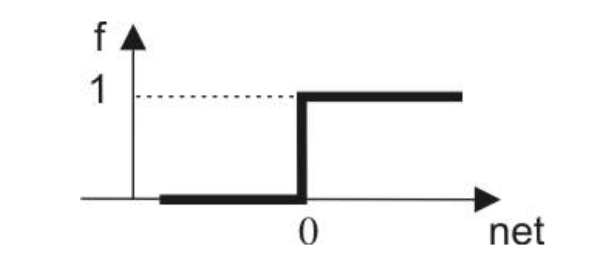
\includegraphics[width=8cm]{img/TLU.png}
\caption{Funkcija skoka}
\label{img:tlu}
\end{figure}

Znak nejednakosti u funkciji skoka, dodatno može u nekim slučajevima sadržavati i znak jednakosti čime se funkcija \ref{eq:tlu} mijenja u \ref{eq:linear-tlu}

\begin{equation}
f(net)=\left\{
\begin{array}{c l}	
     0   & $\textit{za net} $ \leq $ $ a,\\
     net & $\textit{za a} $ < $ \textit{net} $ < $ $ b,\\
     1   & $\textit{za net} $ \geq $ $ b
\end{array}\right.
\label{eq:Funkcija skoka koja je na dijelovima linearna}
\end{equation}

\begin{figure}[H]
\centering
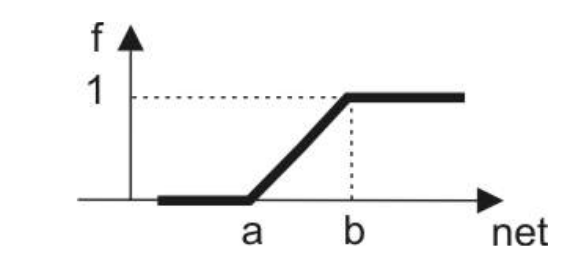
\includegraphics[width=8cm]{img/LinearTLU.png}
\caption{Na dijelovima linearna TLU}
\label{img:linear-tlu}
\end{figure}

Najčešća aktivacijska funkcija jest sigmoida. Vrlo važno svojstvo ove funkcije koje ju razlikuje od dosad navedenih funkcija jest da je derivabilna. To će se pokazati kao vrlo važna značajka za proces učenja neuronske mreže. Sigmoida je definirana kao:

\begin{equation}
f(net) = \frac{1}{1 + e^{-a net}}
\label{eq:sigmoid}
\end{equation}

\begin{figure}[H]
\centering
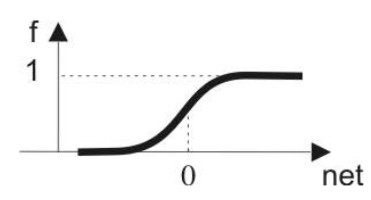
\includegraphics[width=8cm]{img/Sigmoid.png}
\caption{Sigmoidlana (logistička) funkcija}
\label{img:sigmoid}
\end{figure}

gdje parametar $a$ određuje nagib funkcije. Vrlo važno svojstvo sigmoide je da sve brojeve iz bilo kojeg intervala preslikava na raspon $[0,1]$. Zbog toga vrlo često izlaz iz logističke funkcije ima vjerojatnosnu interpretaciju, odnosno koristi se kada je na izlazu potrbno predvijeti vjerojatnosti. Važno je napomenuti da se sigmoida u području strojnog učenja koristi kada model ima binarni izlaz (predviđa 2 klase), dok se za višeklasnu regresiju/klasifikaciju koristi softmax:

\begin{equation}
f(net) = \frac{e^{net_i}}{\sum_{j=1}^{k} e^{net_j}}
\label{eq:sigmoid}
\end{equation}

\begin{figure}[H]
\centering
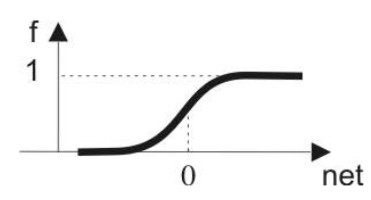
\includegraphics[width=8cm]{img/Sigmoid.png}
\caption{Sigmoidlana (logistička) funkcija}
\label{img:sigmoid}
\end{figure}

Softmax je generalizirana sigmoida. Izlaz iz funkcije softmax također vrlo često ima vjerojatnosnu interpretaciju. 

Zadnja aktivacijska funkcija koju ovdje valja spomenuti je ReLU (\textit{engl. Rectified Linear Unit}). 

\begin{equation}
f(net) = max(0, net)
\label{eq:relu}
\end{equation}

\begin{figure}[H]
\centering
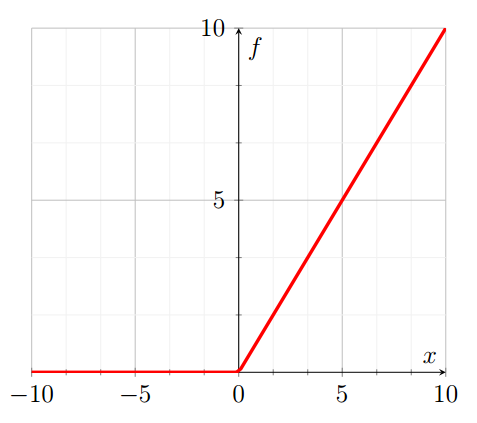
\includegraphics[width=8cm]{img/ReLU.png}
\caption{ReLU}
\label{img:relu}
\end{figure}

Ova aktivacijska funkcija je vrlo raširena u računalnom vidu i vrlo popularna kod konvolucijskih neuronskih mreža. Problem je što ova funkcija sve negativne vrijednosti stavlja u $0$ što smanjuje mogućmost modela da potpuno izvuče znanje iz podataka. Zato je osmišljena još jedna funkcija koja ne preslikava negativne vrijednosti u 0, nego u neku vrijednost blizu $0$ (što je vrijednost negativnija, preslikava se u vrijednost dalje od $0$). Ta funkcija naziva se "Leaky ReLU":

\begin{equation}
f(net)=\left\{
\begin{array}{c l}	
     a {net}   & $\textit{za net} $ < $ $ 0,\\
     {net}     & $\textit{za net} $ \geq $ $ 0
\end{array}\right.
\label{eq:Leaky ReLU}
\end{equation}

\begin{figure}[H]
\centering
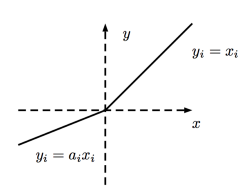
\includegraphics[width=8cm]{img/LeakyReLU.png}
\caption{Leaky ReLU}
\label{img:Leaky ReLU}
\end{figure}

\subsection{Backpropagation algoritam}

Kako bi neuronska mreža mogla predstaviti visoko nelinearne
funkcije, potrebno je da prijenosna funkcija njezinih procesnih elemenata i sama bude
nelinearna funkcija svojih ulaza. Nadalje, radi primjene gradijentne metode pri postupku
učenja mreže, potrebno je da prijenosna funkcija bude derivabilna funkcija težinskih
faktora. Backpropagation algoritam \citep{Backpropagation} nastao je 1970ih godina te omogućuje učenje višeslojnih neuronskih mreža.

Algoritam koristi metodu gradijentnog spusta kako bi minimizirao nastalu pogrešku.
Kod višeslojne mreže izlazni sloj može sačinjavati veći broj neurona, te je potrebno
proširiti definiciju pogreške za višestruke izlaze:

\begin{equation}
E(\vec{w}) = \frac{1}{2} \sum_{d \in D}^{} \sum_{k \in outputs}^{} (t_{kd} - o_{kd})^2
\label{eq:loss-function}
\end{equation}

pri čemu su $t_{kd}$ i $o_{kd}$ ciljna i stvarna izlazna vrijednost za $k$-ti neuron izlaznog sloja dobivene s primjerom za učenje $d$. Učenje višeslojne mreže backpropagation algoritmom svodi se na pretraživanje u n-dimenzionalnom prostoru hipoteza, gdje je n ukupan broj težinskih faktora u mreži. Pogrešku u takvom prostoru možemo vizualizirati kao hiper-površinu koja, za razliku od paraboličke površine jednog procesnog elementa, može sadržavati više lokalnih minimuma u kojima gradijentni spust može zaglaviti. No, u praksi se pokazalo da algoritam daje vrlo dobre rezulatate. Također, postoje i poboljšanja algoritma dodavanjem momenta inercije \citep{NesterovMomentum}.\\

\begin{algorithm}[H]
\caption{Backpropagation algoritam}
\SetAlgoLined
%\KwResult{Write here the result }
 inicijalizacija težina na male slučajne vrijednosti\;
 \While{ $\Delta \varepsilon < \varepsilon_{thresh}$ }{
  izračunaj $o_{i}$ za svaku ulaznu jedinicu $x_{i}$ ulaza $\mathbf{X}$\;
  za svaki izlazni čvor $k$ izračunaj pogrešku $\delta_{k}$
  \begin{equation}
	\delta_{k} \leftarrow o_{k} (1 - o_{k})(t_{k} - o_{k})
	\label{eq:output_unit_loss}
  \end{equation}
  za svaku skrivenu jedinicu $h$ izračunaj pogrešku $\delta_{h}$
  \begin{equation}
	\delta_{h} \leftarrow o_{h} (1 - o_{h}) \sum_{s \in Downstream(h)}^{}(\omega_{hs}\delta_{s})
	\label{eq:hidden_unit_loss}
  \end{equation}
  ažurirati sve težine $\omega_{ij}$
  \begin{equation}
	\omega_{ij} \leftarrow \omega_{ij} + \Delta\omega_{ij}
	\label{eq:update_weights}
  \end{equation}
  gdje je 
  \begin{equation}
	\Delta\omega_{ij} \leftarrow \eta \delta_{j} x_{ij}
	\label{eq:weight_update}
  \end{equation}
 }
 \label{alg:backprop}
\end{algorithm}

Zato što primjeri za učenje određuju ciljne vrijednosti samo izlaznog sloja neurona, poznata nam je jedino pogreška izlaznog sloja \ref{eq:loss-function}. Javlja se pitanje: kako ažurirati težine u skrivenom sloju? Backpropagation algoritam računa pogrešku bilo kojeg skrivenog neurona $h$ tako da zbraja pogreške $\delta$ s svih onih neurona s na koje utječe izlaz neurona $h$, uz dodatno množenje težinskim faktorom $\omega_{hs}$. Faktor ukazuje na to u kojoj je mjeri skriveni neuron $h$ pridonio nastanku pogreške na izlazu jedinice $s$. Skup $Downstream(h)$ jest skup svih neurona "nizvodno" od neurona $h$, tj. svi oni neuroni čiji ulazi uključuju izlaz iz neurona $h$.